% !TeX root = ../SPL-Rules.tex
% !TeX spellcheck = en_US
\section{Forbidden Actions and Penalties}
\label{sec:forbidden_act}

The following actions are forbidden.
In general, when a penalty applies, the robot shall be replaced, not the ball.

\subsection{Penalty Procedure}
\label{sec:penalty_procedure}

When a robot commits an infraction, the head referee shall call out the \textbf{infraction} committed, the \textbf{primary jersey color} of the robot, and the \textbf{jersey number} of the robot.
The penalty for the infraction will be applied immediately by an assistant referee.
The assistant referees should perform the actual movement of the robots for the penalty so that the head referee can continue focusing on the game.
The operator of the GameController will send the appropriate signal to the robots indicating the infraction committed.

For penalties that are timed, the penalty time is considered to be over at the end of each half.

\subsection{Standard Removal Penalty}
\label{sec:removal_penalty}

Unless otherwise stated, all infractions result in the removal of the infringing robot from the field of play for a particular amount of time, after which it will be returned to the field of play.
This process is called the \textit{standard removal penalty}.

When the head referee indicates an infraction has been committed that results in the standard removal penalty, the assistant referee closest to the robot will remove the robot immediately from the field of play.
The robot should be removed in such a way as to minimize the movement of the other robots and the ball.
If the ball is inadvertently moved when removing the robot, the ball should be replaced to the position it was in when the robot was removed.

The GameController will send the appropriate penalty signal to the robot indicating the infraction committed.
After a penalty is signaled to the robot, it is not allowed to move in any fashion (except for standing up).
The removed robot will be placed outside the field facing away from the field of play.

The initial duration of the standard-removal-penalty-time is \qty{\StandardPenaltyTime}{\second}.
Unless otherwise specified, the penalty time increases by \qty{\StandardPenaltyIncrease}{\second} each time a team commits any infraction.

During the \texttt{set} state the penalty time counter will not decrease.

The GameController will keep track of the time of the penalty.
The operator of the GameController will signal the assistant referees when the penalty is \qty{10}{\second} from being over, so that one of them can place the robot in the half of the field which this robot's team is defending on the touchline that is farther from the ball.
The robot should be placed close to the position where the penalty point projects on the touchline.
This is illustrated in \cref{fig:penalty_re-entry_points}.

If there is another robot already in this position, the robot should be replaced at a nearby location along the touchline.
When finding a nearby location, locations away from the ball should be preferred, but they \textbf{must} still be in the robot's own half, so that the symmetry of the field can be resolved by the robot's localization system.

With approximately \qty{5}{\second} left before the penalty ends, the robot should be turned to face towards the opposite touchline.

\begin{figure}[t]
  \centerline{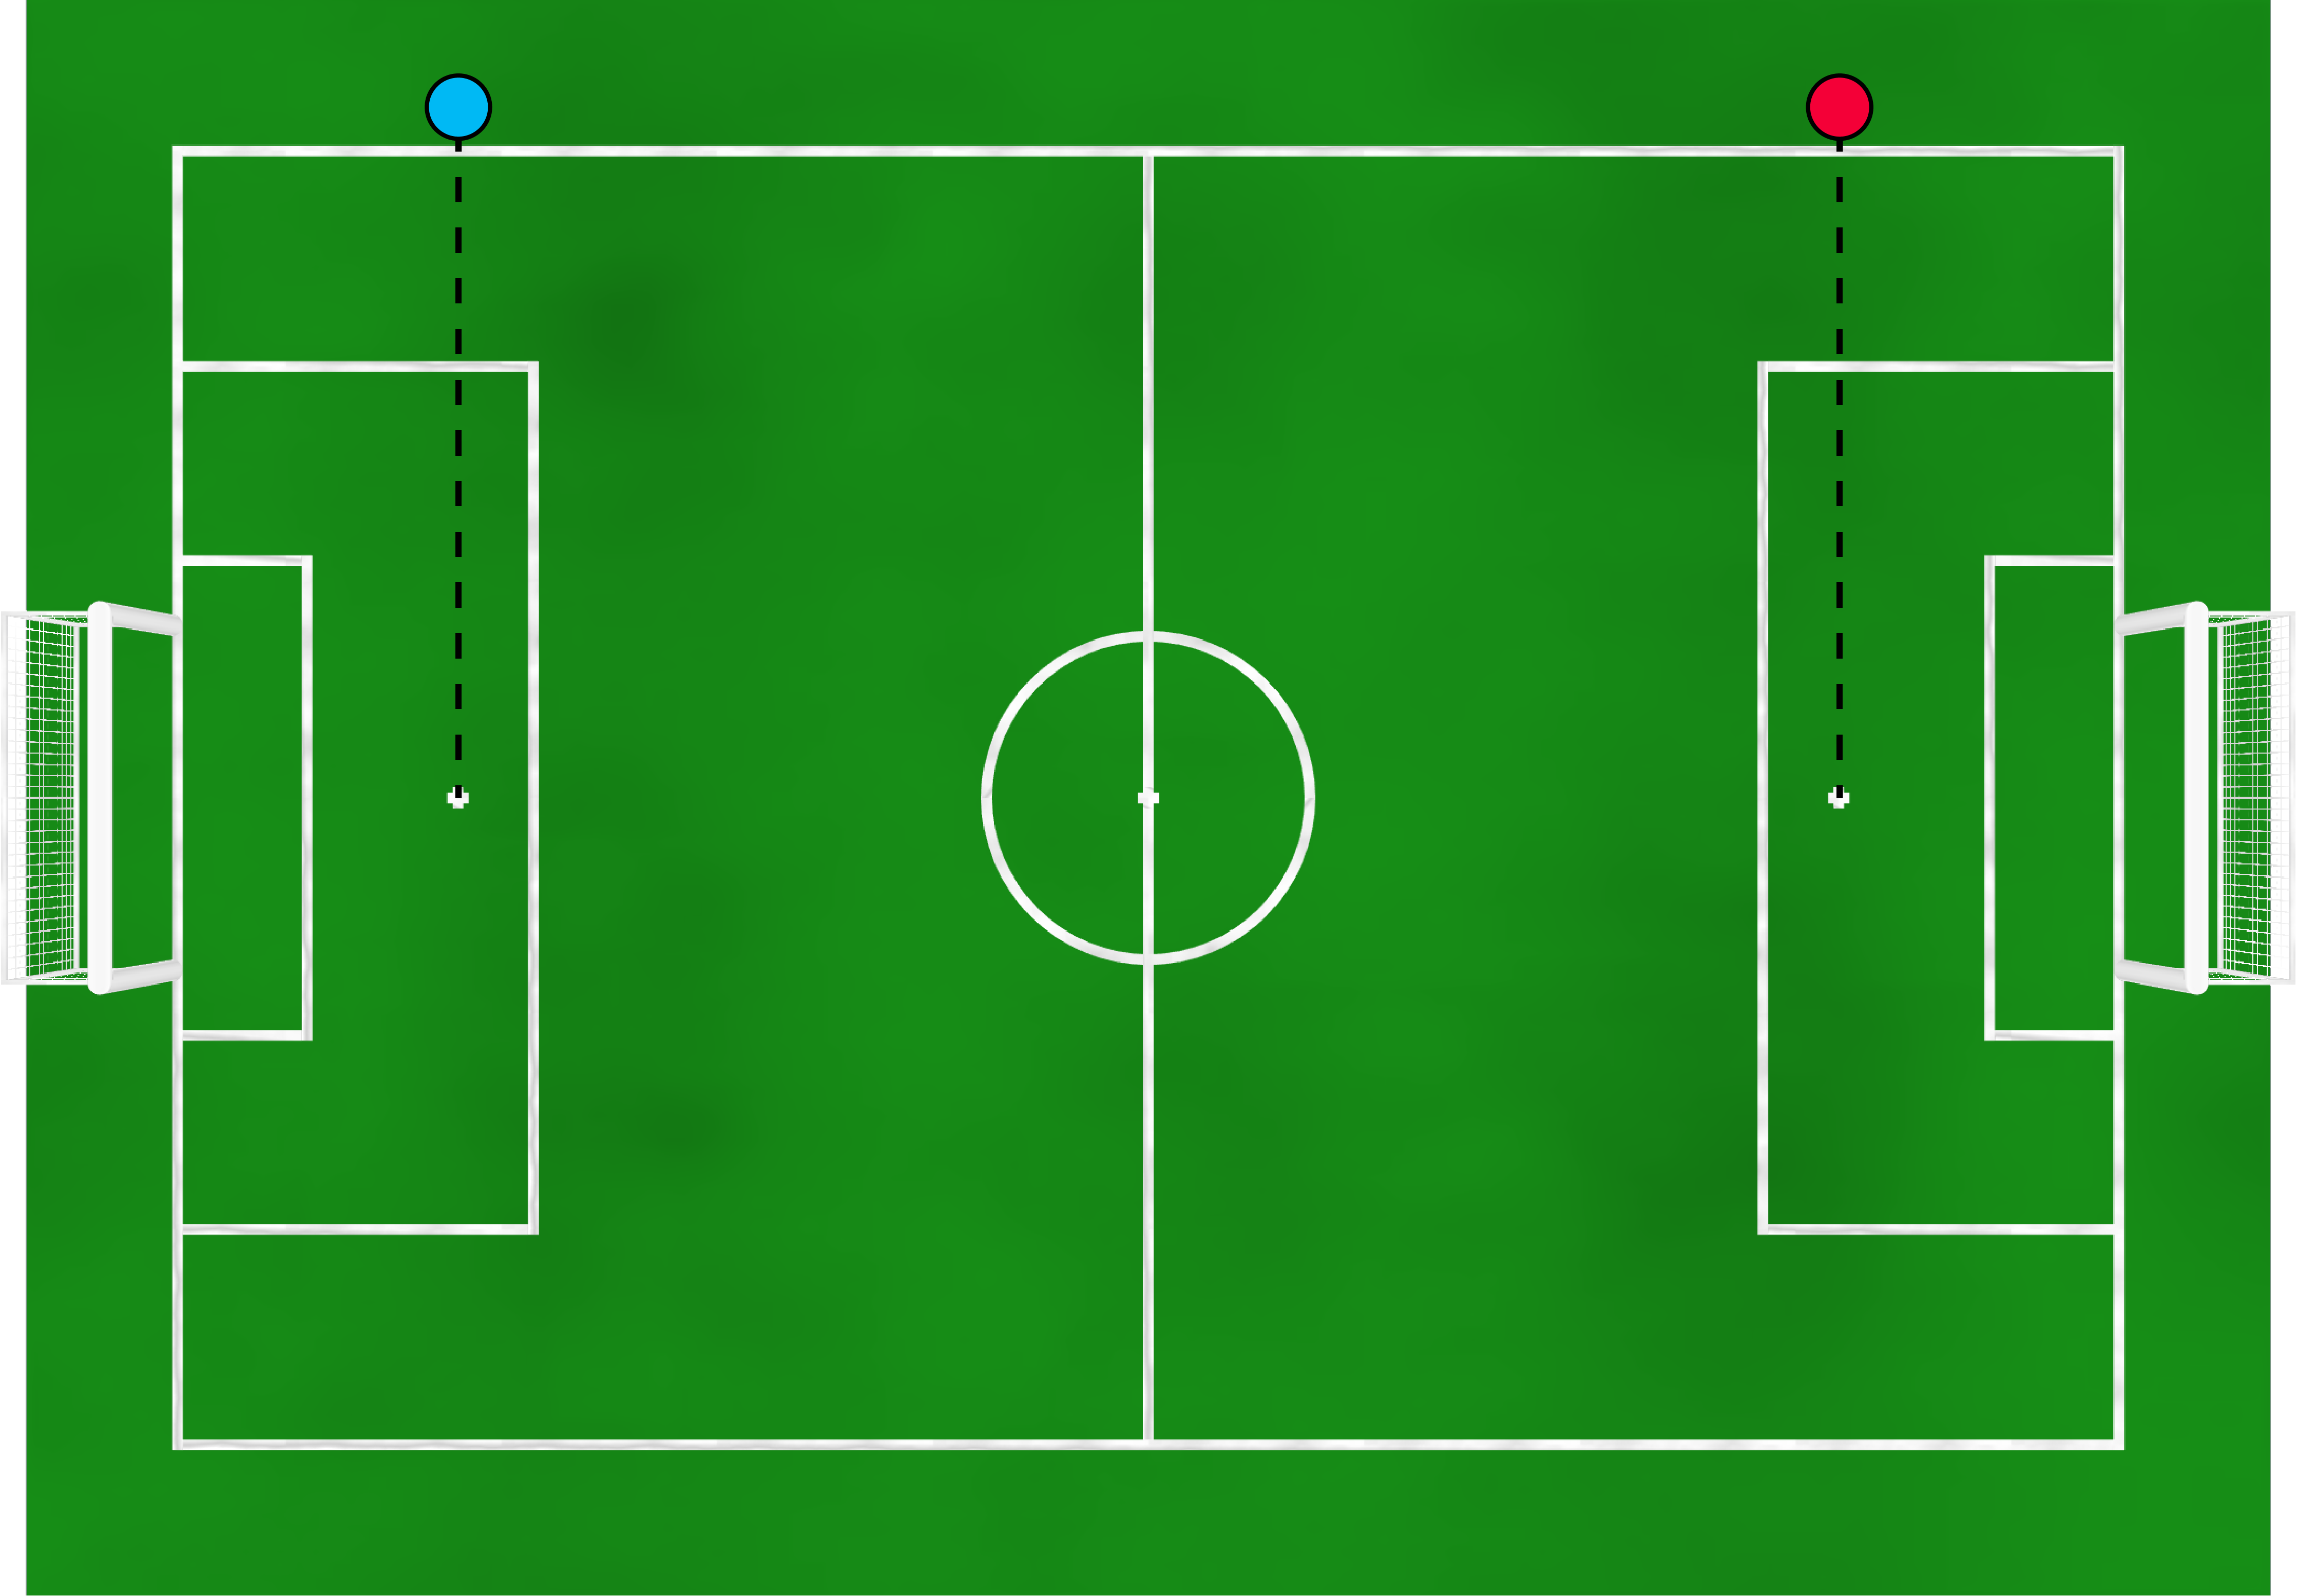
\includegraphics[width=\columnwidth]{figs/penalty_re-entry_points_2020.png}}
  \caption{For robots coming back from a standard removal penalty, re-entry points are in line with the penalty mark in their own half, on the touchline on the side away from the ball.}
  \label{fig:penalty_re-entry_points}
\end{figure}

When the robot is on the field again, the operator of the GameController will send the \texttt{playing} signal to it.

\subsection{Forbidden Actions}

The following actions are forbidden, but not treated as penalties.
Each forbidden action specifies the actions to be taken by the referees.

\subsubsection{Manual Interaction by Team Members}

Manual interaction with the robots, either directly or via some communications mechanism, is not permitted.
Team members can only touch one of their robots when an assistant referee hands it over to them after a ``Request for Pick-up''.

\subsubsection{Damage to the Field}
\label{sec:damage}

A robot that damages the field, or poses a threat to spectator safety, will be removed from the field for the remainder of the game.

\subsection{Illegal Positioning}
\label{sec:illegal_positioning}

A robot penalized under illegal position has the ``Illegal Position'' penalty applied.
Illegally positioned robots are subject to the standard removal penalty (\cf \cref{sec:removal_penalty}).
The head referee will call ``Illegal Position  \textless robot\textgreater''.
Referees may interchange ``Illegal Position'' with ``Illegal Defender'' to help with clarity.

Illegal positions are descried below.

For simplicity, Illegal Positioning penalties during the \texttt{set} state (for kick-off or a penalty kick) do not count towards the incremental penalty count.

Refer to \cref{sec:inside_outside} for the definition of \textit{inside/outside} of a region of the field.

\subsubsection{Before and During Kick-off}
\label{sec:ip_kick_off}

If a robot violates the positioning restrictions made in \cref{sec:kick-off} at the time the \texttt{set} state starts, it will be penalized and removed for \qty{15}{\second}.
If a robot enters the areas of the other team before the ball is in play, it will be penalized and removed according to the standard removal penalty.

\subsubsection{Own Goal Area}
\label{sec:ip_own_goal_area}

During the \texttt{set} and \texttt{playing} states, at most \textit{three} players can be within their own goal area at the same time.

A robot is within the goal area if any part of its body is touching the ground inside the goal area or touching one of its lines.
The penalty is applied when any additional players enter the area in \texttt{playing}, or to the excessive players closest to the border of the goal area in \texttt{set}.
Note that if a player is pushed into the goal area by an opponent, this robot will not be subject to removal, unless it fails to exit the area within \qty{5}{\second} (or \qty{5}{\second} after getting up if the pushing led to falling).

If an illegal defender kicks an own goal, the goal is scored for the opponent.
If there is any doubt about whether a goal should count (\eg the illegal defender infraction is called, but the robot scores the own goal immediately afterwards, before it is removed) then the decision shall be against the infringing robot.

\subsubsection{Defender Encroachment During Free Kick}
\label{sec:ip_free_kick}

If a robot of the defensive team enters or does not attempt to leave the circular area with \qty{\FreeKickRadius}{\metre} radius around the ball after a free kick (\cf \cref{sec:free_kick}) was called, ``Illegal Position'' is called.
Note that the referee should not look for exact distances and rather penalize only those robots who clearly violate this rule.
As a guideline, the robots of the defensive team should clear the ball within \qty{10}{\second}.

\subsubsection{Penalty Area During Penalty Kick}
\label{sec:ip_penalty_kick}

If a robot enters the relevant penalty area during a penalty kick, except for the goalkeeper (defending team) and one robot of the attacking team, ``Illegal Position'' is called.

\subsection{Motion in Set}
\label{sec:motion_in_set}

Robots that begin moving their legs or locomote in any fashion during \texttt{set} (\ie before the head referee blows the whistle) will be penalized \textit{in place} on the field for \qty{15}{\second}.
The head referee will call ``Motion in Set \textless robot\textgreater''.
``Motion in Set'' penalties do not follow the standard removal procedure, and hence do not count towards the incremental penalty count.
A robot will be moved back to its original position if it has moved significantly before becoming penalized.
Note that responding to a whistle on another field will result in this penalty.

\subsection{Fallen or Inactive Robots}
\label{sec:fallenrobots}

If a robot falls during the game, it should start executing a get-up action within \qty{5}{\second}.
If it does not commence a get-up action within \qty{5}{\second}, it will be penalized and removed for \qty{45}{\second}.
A fallen robot which is unable to autonomously stand up within 2 attempts, or 3 if disturbed externally during the first two attempts, will be penalized and removed for \qty{45}{\second}.
In both cases, the head referee will call ``Fallen Robot  \textless robot\textgreater''.
The goalkeeper, inside its own penalty area, is the only robot permitted to `dive' (that is deliberately falling in a way that might cause its torso, arms, or hands) to intercept the ball.
In all other cases, the robot should remain upright---that is, supported by its feet.

A robot that has ceased activity for \qty{10}{\second} or has turned off will be removed and penalized for \qty{45}{\second}.
The head referee will call ``Inactive Robot \textless robot\textgreater''.
A robot is active if it performs at least one of the following:
\begin{enumerate}
  \item The robot walks in any direction, or turns.
  \item The robot searches for the ball, or is looking at the ball.
\end{enumerate}

Fallen/Inactive Robot penalties do not follow the standard removal procedure, and hence do not count towards the incremental penalty count.

\paragraph{Note:} The intention of this rule is not to penalize robots simply for being stationary---provided they are not `asleep' and have not `crashed'.

\subsection{Local Game Stuck}
\label{sec:pen_local_game_stuck}

When Local Game Stuck is called, the nearest robot to the ball will be penalized and removed for \qty{45}{\second}.
Local Game Stuck penalties do not follow the standard removal procedure, and hence do not count towards the incremental penalty count.

\subsection{Ball Holding}
\label{sec:ball_holding}

The goalkeeper is allowed to hold the ball for up to \qty{10}{\second} as long as it has one foot inside in its own penalty area.
In all other cases (except those noted in \cref{sec:situations_no_ball_holding}), robots are allowed to hold the ball for up to \qty{3}{\second}.
Holding the ball for longer than this is not allowed.
The head referee will call ``Ball Holding \textless robot\textgreater'', and the robot removed under the standard removal penalty.
The ball should be removed from the possession of the robot and placed where the penalty occurred.
If the robot that held the ball has moved the ball before the robot can be removed, the ball shall be replaced where the penalty occurred.
This applies to accidental goals.

\textbf{Example.} A robot holds the ball, and before the referees can remove the robot, it shoots the ball into the goal.
The goal will not be counted, and the ball will be replaced where the penalty occurred.

A robot must leave enough open space around the ball.
The occupation of the ball is judged using the convex hull of the projection of the robot's body onto the ground.
``Enough open space'' means that at least the half of the ball is not covered by the convex hull.
It is not important whether the robot actually touches the ball.

\begin{figure}[t]
  \centerline{\begin{tabular}{ll}
  a) & b) \\
  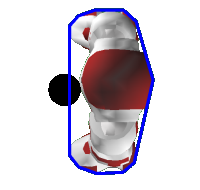
\includegraphics[scale=0.7]{figs/holding1} &
  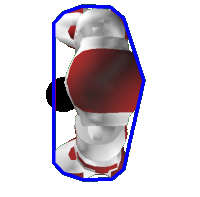
\includegraphics[scale=0.7]{figs/holding4}
  \end{tabular}}

  \caption{Examples for ``Ball Holding''. The black circle is the ball and the blue polygon visualizes the convex hull of the robot's projection onto the ground. Situation a) is legal, whereas b) violates the rule.}
  \label{fig:holding}
\end{figure}

Intentional continual holding is prohibited even if each individual holding time does not continue for up to the time limit.
In general, robots should release the ball for approximately as long as they were holding it to reset the clock.
Without a sufficient release, the continual holding is regarded as a continuous hold from the very beginning and the holding rule is strictly applied.

\subsubsection{Exceptions to the Ball Holding Rules}
\label{sec:situations_no_ball_holding}

The following define situations where ball holding does not apply:
\begin{enumerate}
  \item Ball holding may not occur when the ball becomes stuck between a robot's legs.
    In such a situation, the head referee should call `clear ball' and an assistant referee should remove the ball and place the ball approximately where it was before it became stuck.
  \item Ball holding may not occur when a robot falls on a ball.
    The robot will either get up and hence free the ball, or the robot should be removed under the Fallen Robot rule.
\end{enumerate}

\subsection{Player Stance}
\label{sec:player_stance}

Robots are not allowed to stay in a stance that is significantly wider than the width of the robot's shoulders for more than \qty{5}{\second}.
Staying in a wide stance for longer than \qty{5}{\second} will result in the standard removal penalty.

This rule applies to upright robots only, \ie robots that are supported by their feet.
Other cases are handled by the fallen robot rule (\cf~\cref{sec:fallenrobots}).

\subsection{Player Pushing}
\label{sec:player_pushing}

% basic definition of pushing
\emph{Pushing} is a direct or indirect forceful contact with any other opponent robot, \ie, enough to destabilize it, and is not allowed.
In the following, exceptions to this rule are specified in more detail.
The head referee will call ``Pushing \textless robot\textgreater''.

If the ball moves significantly as the result of pushing, then it should be replaced to where it was at the time of the infraction.

A \textbf{Pushing Free Kick}, see~\cref{sec:free_kick}, is awarded against the robot penalized for pushing
\begin{itemize}
  \item[1.] if the robot is in an approximately \qty{0.5}{\metre} radius around the ball and
  \item[2.] if the pushed robot was \textbf{not} inside the penalty area of the pushing robot.
\end{itemize}

A \textbf{Penalty Kick}, see~\cref{sec:penalty_kick}, is awarded against the robot penalized for pushing
\begin{itemize}
  \item[1.] if the robot is in an approximately \qty{0.5}{\metre} radius around the ball and
  \item[2.] if the pushed robot was inside the penalty area of the pushing robot.
\end{itemize}

The following exceptions define situations where pushing does not apply:
\begin{itemize}
  \item Pushing may occur \textbf{only} between players of different teams.
  \item A stationary robot cannot be penalized for pushing, including a robot that is kicking, provided that the ball was close enough where a kick could have succeeded at the start of the kick motion.
  \item A robot currently getting up cannot be penalized for pushing.
  \item The goalkeeper cannot be penalized for pushing while looking at or chasing the ball in its own penalty area.
  \item Front to front contact between robots with the ball between them does not constitute pushing.
  \item Any robot proceeding to the ball whose side (\ie arm, shoulder etc.) makes contact with another robot cannot be called for pushing, even if the second robot is not proceeding to the ball.
  \item A robot pushed by another robot cannot simultaneously be called for pushing itself.
    Only the robot, who initially pushed the other robot, will be called for pushing.
\end{itemize}

\subsection{Playing With Arms/Hands}
\label{sec:hand_ball}

Playing with arms/hands occurs when a field player or a goalkeeper outside its own penalty area moves its arms/hands to touch the ball (except during a fall or get-up).
The goalkeeper is allowed to touch the ball with its arms/hands while it is within its own penalty area.
A robot playing with arms/hands will be subject to the standard removal penalty and the ball will be replaced at the point where it contacted the arms/hands of the offending robot.
If an own goal is scored as a result, the goal should count and the player should not be penalized.

Accidental playing with arms/hands when a robot falls or executes a get-up routine will not be penalized.
If the ball goes out of play in this case, normal kick-in rules will apply (\cf \cref{sec:kick_in}).
However, goals (except for own goals) resulting from a ball contact with the arms/hands during a fall or get-up do not count and result in a Goal Kick (\cf \cref{sec:free_kick}) as if the ball went over the goal line next to the goal.

\subsection{Leaving the Field}
\label{sec:leaving_field}

A robot that intends to leave the \qty{\TotalWidth}{\metre} $\times$ \qty{\TotalLength}{\metre} carpeted area will be subject to the standard removal penalty (\cf \cref{sec:removal_penalty}).
The head referee will call ``Leaving the Field \textless robot\textgreater''.

Additionally, a robot will also be subject to the standard removal penalty, when:
\begin{itemize}
  \item The robot walks into the goalposts or goal net for more than \qty{5}{\second}, this includes robots that are stuck on the goalposts and unable to free themselves.
  \item The robot's fingers become entangled in the net (without any time constraint).
\end{itemize}

\subsection{Jamming}
\label{sec:jamming}

During a match, any robot shall never jam the communication and the sensor systems of the opponents:
\begin{description}
  \item[Wireless communication.] Each robot is only allowed to send a limited number of UDP messages that have to comply with a predefined format (\cf \cref{sec:wireless}).
    If a robot uses a different protocol or sends too much data in a game, penalties will apply.
    If a team violates this rule in multiple games, disqualification from the tournament (including all technical challenges and side competitions) as well as an entry in the penalty list will be the consequence.
    Except for the wireless cards and the access points provided by the organizers of the competition, nobody close to the field is allowed using \qty{2.4}{\giga\hertz} or \qty{5}{\giga\hertz} radio equipment (including cellular phones and/or Bluetooth devices).
  \item[Whistle interference.] Both the teams and the audience shall avoid intentionally confusing the robots by producing similar sounds to the game whistle.
  \item[Acoustic communication.] If acoustic communication is used by both teams, they shall negotiate before the match how they can reduce interference.
    If only one team uses acoustic communication, the robots of the other team shall avoid producing any sound.
    In addition, both the teams and the audience shall avoid intentionally confusing the robots by producing similar sounds to those used for communication.
  \item[Infrared communication.] If infrared communication is used by both teams, they shall negotiate before the match how they can reduce interference (if at all).
    Both the teams and the audience shall avoid confusing the robots by producing similar infrared signals to those used for communication.
  \item[Visual perception.] The use of flashlights is not allowed during the games.
    However, flash photography from the audience is allowable as long as the head referee believes the purpose of the flash is not to jam any of the robots.
\end{description}
